%------------------------------------------------------------------------------
% 
\chapter{Real World Knowledge Acquisition Implementation}
\label{chapter:implementation}
%-------------------------------------------------------------------------------
This chapter presents the actual implementation in the system described
in the previous chapters (especially in \autoref{chapter:approach}). While up 
to now we've been describing the idea and a general approach to do it 
(independent of the implementation), here we represent the actuall working
system that we implemented and kept it online in the shape of the current 
version since the end of 2012. 

\begin{figure}[H]
	\centering
		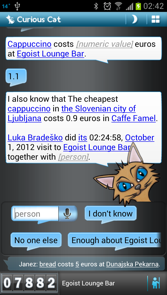
\includegraphics[width=0.41\textwidth]{figures/androidExample.png}
	\caption{Screenshot of Curious Cat Android app.}
	\label{fig:androidExample}
\end{figure}

During this time, 5,185 users installed its
client app, out of which 2,401 users registered, and 1,715 users used it at 
least once (see the results chapter, \autoref{section:stickiness} for more 
details on users).
The development  of \emph{Curious Cat} implementation started on October 
26th, 2010 and halted on June 2014. The
implementation follows closely the architecture presented on 
\autoref{fig:Architecture} in \autoref{chapter:approach}. For the core
of the system we took Cyc with its common sense KB and inference engine, which 
was also an initial inspiration for the development and the approach, where
the main work needed to be done on the part of the meta-KB and also common
sense KB extensions to support our use-cases. For the NL modules, our 
implementation relies on the internal Cyc logic to NL conversion modules, and
on SCG\parencite{Schneider2015}. The procedural component and client were 
written from scratch. All together our implemented system consists of 50,686
lines of Java source code, and 12,616 lines of knowledge definitions (8,571) for
the additional knowledge we added in CycKB to drive our KA process.

Besides the implementation described here, this system was also implemented and
deployed as a real-time commuting companion\parencite{Figueiras2013}, and as an
RDF framework for on the field sensor information knowledge acquisition
\parencite{Bradesko2012a}. Commuting companion implementation and this implementation
were also described in the books \emph{Intelligent Decision Technology 
Support in Practice}\parencite{Costa2016} and \emph{Handbook of Human 
Computation}\parencite{Witbrock2013}. This implementation was also mentioned
in the \emph{Communications of the ACM} magazine article\parencite{Geller2016}.

Implementation consists of Android based mobile client (see screenshot on
\autoref{fig:androidExample}), Java Servlet based
\emph{Procedural Component} with PostGreSQL database access, two Research 
Cyc instances 
(KB, Inference Engine, NL Conversion) to increase the speed and reliablility 
of the system, \emph{Transcript Server} for syncing between Cyc instances, 
and a web-site for registration and email confirmation. This organization is 
also depicted on \autoref{fig:implementation} below.

\begin{figure}[H]
	\centering
		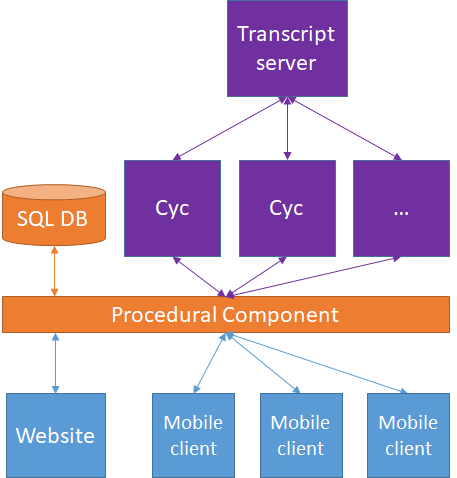
\includegraphics[width=0.62\textwidth]{figures/implementationOrg.png}
	\caption{Organization of the system modules in our implementation.}
	\label{fig:implementation}
\end{figure}

\section{Cyc}
\label{section:Cyc}
As already mentioned in related work (\autoref{section:relatedCyc}), \emph{Cyc}
is an AI project started in 1984 by Douglas Lenat\parencite{Lenat1985} with the
premise, that in order to make computers think like humans do, we need to first
make sure that they have same common sense knowledge as humans do. Since then,
\emph {Cyc} team (now part of \emph{Cycorp Inc.}), is codifying and entering 
the knowledge by hand and also by other means of knowledge acquisition and 
mining (see rows stating "Cyc" as parent in \autoref{tab:related}, 
\autoref{chapter:related} - \nameref{chapter:related}). 
The collected and codified knowledge is represented in machine-usable form 
using emph{CycL (Cyc Language)}, and is structured and grouped together as
\emph{CycKB}. In parallel with the KB, Cyc also contains an inference engine
that works on the scale of the KB, and a set of tools, APIs and other interfaces
for interacting with the system, ranging from web interface, natural language,
web APIs and also Java interfaces, which we used in our implementation and
communication with the procedural part of our system 
(\autoref{section:prophet}).

%subsection
\subsection{Cyc KB}
\label{section:cyckb}
At this moment (end of 2017), \emph{Research CycKB} consists of more than 
630,000 concepts, 7,000,000 assertions (rules are also assertions), made with
using more than 38,000 predicates (relations), covering a broad domain of
human common sense knowledge. The KB is divided into thousands of microtheories
(not counting the microtheories we added for \emph{CC} implementation - 
\autoref{section:crowdsourcing}), where each microtheory is a set of assertions
that share common assumptions. Microtheories (Mts) can hierarchically stack on 
top of each other and allow \emph{Cyc} to independently maintain assertions that
could contradict each-other. This also enhances the performance of the 
\emph{Cyc} inference engine, since it can be limited on one particular, or a
group of Mts to limit the number of facts it needs to use while inferencing.

\emph{CycKB} is represented in \emph{CycL}, with most basic syntax described as:
\begin{itemize}
\item Logical constants are represented by "$\#\$$" sign, followed by the name 
of the term name ($\#\$JoesPizza$).
\item Formulas are enclosed in parentesis. If more than one constants or terms
are part of the assertion, the predicate is always first, followed by its
arguments, for example: $(\#\$menuItem\quad\#\$JoesPizza\quad\#\$Pizza)$
\item Variables are represented by the question mark ("$?$") sign, followed
by the name in capital ($?PERSON$). For example, query asking the inference
engine, what is on the menu in Joe's Pizza is represented as: 
$(\#\$menuItem\quad\#\$JoesPizza\quad?ITEMS)$, where the name of the variable
"ITEMS", can be arbitrary.
\end{itemize}
%subsubsection
\subsubsection{CC KB}
\label{section:cckb}
dada

%subsection
\subsection{Cyc Inferene Engine}
\label{section:cycinference}
dada

%subsection
\subsection{Transcript server}
\label{section:transcriptserver}
TBW

%subsection
\subsection{Cyc NL generation}
\label{section:cycnl}
dada

%subsection
\subsection{SCG}
\label{section:scg}
TBW

%section
\section{Mobile Client}
\label{section:app}
TBW

%section
\section{Procedutal Component}
\label{section:prophet}
dada
